\documentclass[times, 10pt, twocolumn]{article}
\usepackage{latex8}

%\usepackage{times}
%\documentclass[conference]{IEEEtran}

\usepackage[T1]{fontenc}
\usepackage[latin1]{inputenc}

\usepackage{times}
\usepackage{cite}
\usepackage{url}
\usepackage{graphicx}

\begin{document}

\title{Adaptive middleware for opportunistic grid: a mobile agent approach}

\author{Vinicius Pinheiro, Alfredo Goldman\\
Dept. of Computer Science, Universidade de S\~ao Paulo, Brazil\\
\{vinicius,gold\}@ime.usp.br}

\maketitle
\thispagestyle{empty}

\begin{abstract}

The mobile agent paradigm has emerged as a promising alternative to overcome the
construction challenges of opportunistic grid environments. MAG (Mobile Agents
for Grid Computing Environment) explores this powerful paradigm by dynamically
loading sequential grid applications into mobile agents. These MAG agents can
be dynamically reallocated to grid nodes through a transparent migration
mechanism as a way to provide load balancing and support for non-dedicated
nodes. MAG also includes retrying, replication and checkpoint as
fault-tolerance techniques. These mechanisms can be applied in a flexible
manner, since the user can combine them in order to meet different scenarios of
resource availability. In this paper we describe the MAG architecture and what
it can do in a volunteer computing environment. We also propose a
fault-tolerant mechanism based on dynamic task replication and checkpointing in
order to meet different scenarios of resource availability. 
\end{abstract}

%============================================================================

\Section{Introduction}
% TODO missing references 

Opportunistic grids are distributed environments built to leverage the
computacional power of idle resources geographically spread across different
administrative domains. These environments comprise many charateristics such as
high level heterogeneity and variation on resource availability. 

The central element of a opportunistic grid infrastructure is its middleware.
The grid middleware hides the complexity related to distribution and
heterogeneity and must efficiently address several issues, such as management
and allocation of distributed resources, dynamic task scheduling, fault
tolerance, support for high scalability and great heterogeneity of software and
hardware components, protection and security requirements.
 
%These agents can be used to implement
%mechanisms that enable the progress on the execution of applications even in
%the presence of failures.  These mechanisms can be combined in a flexible
%manner to meet different scenarios of resource availability. In this work, we
%describe the architecture of the MAG middleware (Mobile Agents for grid
%Computing Environment) and what it can do in a opportunistic grid environment.
%We use this middleware as a foundation for the proposal of a adaptive fault
%tolerance mechanism based on task replication and checkpointing. Finally, we
%analize experimental and
%simulation results.

In distributed systems such as opportunistic grids, failures can occur due to
several factors, most of them related to the resources heterogeneity and
distribution. These failures among with the usage of the resources by its
owners modify the availability status of the resources in the grid (i.e.
resources can be active, busy, offline, crashed, etc) and the middleware must
monitoring and detect such changes in order to reschedule the applications
among the available resources or dynamically tunning the fault tolerance
mechanisms to obtain a better adequacy to the actual scenario of availability. 

In this work, we implement dynamic fault tolerance mechanism for grid
applications and to do so we rely in the mobile agent paradigm. Mobile agents
are programs that can move from one resource to another in a autonomously way
carrying its data and execution state to resume its execution at the
destination. We argue that these agents exhibits great adequacy for dealing
with the complexity related to the construction of opportunistic grids due to
intrinsic characteristics, such as:

\begin{enumerate}
    \item \emph{Cooperation}: agents have the ability to interact and cooperate
    with other agents; this can be explored for the development of complex
    communication mechanisms among grid nodes;
   
    \item \emph{Autonomy}: agents are autonomous entities, meaning that their
    execution goes on without any or with little intervention by the clients
    that started them. This is an adequate model for submission and execution
    of grid applications;
  
    \item \emph{Heterogeneity}: several mobile agent platforms can be executed
    in heterogeneous environments, an important characteristic for better use
    of computational resources among multi-institutional environments;
  
    \item \emph{Reactivity}: agents can react to external events, such as
    variations on resources availability;
  
    \item \emph{Mobility}: mobile agents can migrate from one node to another,
    moving part of the computation being executed and providing load balancing
    among grid nodes;
  
    \item \emph{Protection and Security}: several agent platforms offer
    protection and security mechanisms, such as authentication, cryptography
    and access control.
\end{enumerate}

Since 2004, our research group has being working on applying the agent paradigm
for developing a grid software infrastructure, leading to the MobiGrid and MAG
projects \cite{barbosa04,lopes05}. The middleware follows an opportunistic
approach, where idle computing power of personal workstations is used for
executing computationally-intensive parallel applications.

Two execution models are supported by the developed infrastructure: regular and
parametric (or bag-of-tasks) model. The parametric model can be applied to a
wide range of grid applications. In this case, multiple copies of a single
binary are executed on different grid nodes. Each process receives a sub-set of
the application input data and carries out its computation in parallel with the
others, without requiring any communication among them.

In this scenario, the likelihood of errors is exacerbated due to several
reasons: each process must successfully finish its execution in order to
generate a successful application execution; grid applications usually perform
complex computations, requiring large execution times; opportunistic grid
environments are very dynamic since the user can request at any time exclusive
use of resources (workstations).

\subsection{Contributions and Paper Organization}

This work describes improvements to the MAG grid middleware for
efficiently addressing the high dynamic of the opportunistic
environments, providing an effective management for long sequential and
parametric applications and the allocation of resources necessary for its
successful execution.

% FIXME rewrite this paragraph.
On the next section we present some of the related work. Then on
Section~\ref{sec:arch} we present the MAG and Integrade architecture. On
Section~\ref{sec:faulttolerance} we present the necessary changes to efficient
support the fault tolerance. We provide some experimental results on
Section~\ref{sec:eval}, and on the last Section we present our conclusions.


%============================================================================

\Section{Related Work}
% Cite UWAgents, CoordAgents e GridWFS (lookup master dissertation)

There are several works that are related to this paper, some related to the
systems giving support for BoT like applications, some related to
running long sequential applications on non-dedicated environments, and finally
some works on the implementation of mobile agents on grid middlewares.

The most well known work was provided by research on extraterrestrial life on
the SETI program~\cite{seti} where more attention were paid on security aspects
and on the reliability of the results. More recently, the BOINC
project~\cite{boinc} proposed an infrastructure allowing the execution of
different programs which can be executed on volunteer computers spread around
the world. There exist similar projects both with a fixed algorithm as
Mersenne~\cite{mersenne}, and where different algorithms or challenges can be
programmed~\cite{distributed}. However, on these projects the support for long
running sequential applications is mostly restricted to local checkpoints (with
few exception like~ \cite{climate}, or the use of replication to guarantee the
progress of the individual applications). Another bag-of-tasks approach is
based on OurGrid~\cite{cirne06}, however the main focus is on dealing with
the middleware infrastructure and not on the individual sequential
applications.

Several works deals with checkpointing techniques to guarantee the progress of
sequential long running applications. One that is directly related to our
work is~\cite{hwang03}. In this work the authors studied several approaches to
deal with failures on machines. The handling techniques were: retrying, checkpointing,
replication, and replication with checkpointing. They concluded that in grid
environments with high down-time, as it can happen in opportunistic environments,
the replication with checkpointing outperforms the other ones, using as comparison
the lower completion time.

Several works present the use of mobile agents on grid environments, some using
opportunistic contexts~\cite{fukuda03}, but most of them presents characteristics
more related to the middleware, not the
application~\cite{cao02,cao01,loke03,martino04}. Some of the mobile agent work
were done within our project Integrade~ \cite{goldchleger04}. The first ideas on
using mobile agents on an opportunistic grid appeared in~\cite{barbosa04} where
an architecture based on Aglets~\cite{aglets} is first presented, and then
evaluated with the use of several replicas in~\cite{barbosa05}. More recently a
work based on the mobile agents framework Jade~\cite{jade} was also
presented~\cite{lopes05,lopes06_2}, where there is application instrumentation, to
provide transparent checkpointing and some work on fault tolerance.

To the best of our knowledge this paper is the first one that
specifically uses mobile agents combined with techniques of
replication and checkpointing, within a grid middleware, to provide
dynamic fault tolerance mechanisms for sequential and parametric applications
on opportunistic environments.

%===========================================================================e

\Section{The middleware MAG}\label{sec:arch}
% TODO include architecture description
% TODO write about JADE
% TODO write about fault-tolerance
% TODO include code examples(optional) and screenshots
% TODO cite CORBA

The Integrade project evolves the development of a grid middleware that
leverages the idle computational power of desktop machines. This project is
maintained by the Institute of Mathematics and Statistics of the University of
S\~{a}o Paulo along with others institutions. InteGrade is based on
CORBA~\cite{vinoski97}, an industry standard for distributed object systems. InteGrade
naming service uses CORBA IDL (Interface Definition Language) being accessible
from a large variety of programming languages and operating systems. The
Integrade architecture follows an hierarchy in which each node can assume
different responsibilities. The Cluster Manager is represented by one or more
nodes that are responsible for managing that cluster and performing
communication with other clusters. A Resource Provider node is the one that
exports part of its resources, making them available to grid users. A User Node
is one belonging to a grid user who submits grid applications. As we can see in
figure \ref{fig:integrade}, Integrade architecture follows a two-tier
intra-cluster hierarchy, and a peer-to-peer based inter-cluster network.

\begin{figure}[th]
\centering 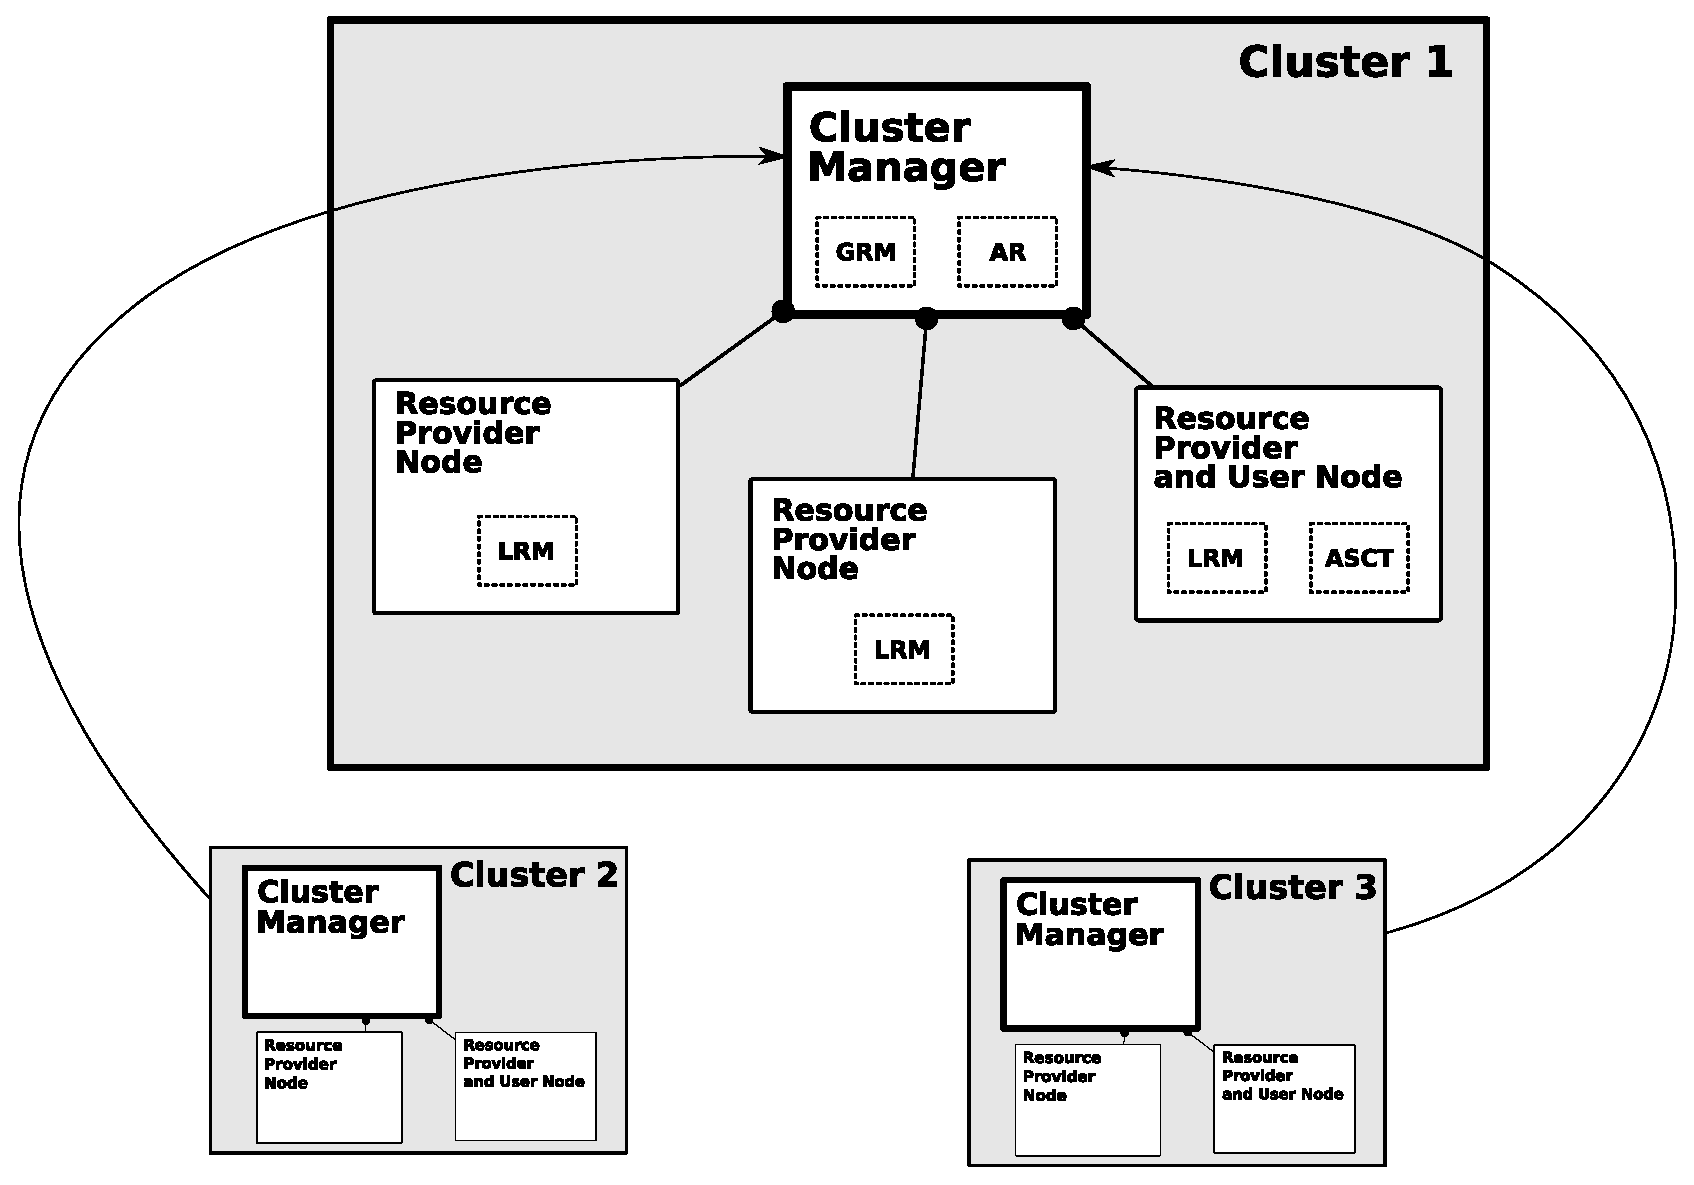
\includegraphics[width=1\columnwidth]{images/integrade2_ieee.eps}
\caption{Integrade architecture}
\label{fig:integrade}
\end{figure}


The MAG project was developed by the Dept. of Computer Science of the Federal
University of Maranh\~{a}o and introduces the mobile agent technology as new way
of executing applications on Integrade. Through MAG, the grid user can submit
Java applications, not supported by the native Integrade middleware. This is
performed by dynamically loading sequential grid applications into mobile
agents. Figure \ref{fig:magarch} depicts the architecture layers of the MAG middleware.
The JADE~\cite{jade} (\emph{Java Agent Development Framework}) layer represents the agent
plataform used by MAG to provide agent services such as communication and life
cycle monitoring. Jade provides a private queue of messages to each agent
allowing them to exchange messages specifying their topics and their receivers.
JADE is portable, since it was implemented in Java, and complies with the
FIPA~\cite{fipa} specification (Foundation for Interlligent Physical Agents).

\begin{figure}[th]
\centering \includegraphics[width=0.7\columnwidth]{images/magarch_en.eps}
\caption{Integrade/MAG middleware layers}
\label{fig:magarch}
\end{figure}


In order to avoid duplication of efforts, the MAG project was build on top of
some Integrade components:

\begin{enumerate}

    \item \emph{Local Resource Manager (LRM)}: This component is executed in
each Resource Provider node, loading the execution environment and wrapping the
application processes delegated to it. LRM also contains a sub-component called
LUPA (Local User Pattern Analyser) that collects informations about memory and
CPU utilization. The LRM sends status information about applications in
execution. It also sends heartbeat messages periodically.

    \item \emph{Global Resource Manager (GRM)}: This is the main component in
the grid and is executed in the Cluster Manager Node. The GRM holds
informations about the registered LRMs and is able to send tasks to them.

    \item \emph{Application Repository (AR)}: This component provides a
centralized repository to store application binaries that will be submitted for
execution.

    \item \emph{Application Submission and Control Tool (ASCT)}: This component
is executed in the User Node and provides a interface in which the user can
submit applications to the grid. The user can also monitoring the execution
status and view the results of the execution.

\end{enumerate}

Besides those, MAG architecture adds some others components that provides
mobile agents capabilities and fault-tolerance mechanisms:

\begin{enumerate}

    \item \emph{ExecutionManagementAgent (EMA)}: This component stores
    informations about current and past executions, as the current execution state
    (accepted, running, finished), input arguments and scheduled machines. This informations
    could be retrieved to restore applications to the point that they were before
    the failure.

    \item \emph{AgentHandler}: This component runs on top of the LRMs. The
    AgentHandler works as a proxy to the JADE agent platform, instantiating
    MAGAgents for each requested execution.

    \item \emph{ClusterReplicationManagerAgent (CRM)}: When the GRM receives a
    execution with replicas request it delegates to the CRM. This component
    processes informations for each replica an create an ERM agent to handle the
    request.

    \item \emph{ExecutionReplicationManagerAgent (ERM)}: This component
    contacts the LRMs of the target machines in order to execute the replicas, one
    in each machine.

    \item \emph{StableStorage}: The stable storage receives the compressed
    checkpoints in order to store them in the file system, and retrieve it when
    receives a query request. This agent runs in the Cluster Manager node.

    \item \emph{MAGAgent}: This is the main component of the MAG middleware.
    The MAGAgent wraps the application, instantiate it, and catch the application
    exceptions that my arise. It also controls the applications life cycle.

    \item \emph{AgentRecover}: This component is created on demand to performs
    the recovery of the execution in the presence of incidental failures.

\end{enumerate}

\subsection{Fault-tolerance in MAG\label{sec:faulttolerance}}

In this section we present the fault-tolerance mechanisms availables on MAG.
This mechanisms can be combined to meet different scenarios of resource
availability, resulting in 4 different strategies:

\begin{enumerate}
    \item \emph{Retrying}: Every time the application fails it is automatically submitted again.
   
    \item \emph{Replication}: Various replicas of the application are submitted
for execution at the same time. When one of the replicas finishes, the others
are discarded to avoid overconsumption of resources. In case of failure,
retrying is applied.
   
    \item \emph{Checkpointing}: The application periodically saves its execution
state in a stable storage. In case of application failure, the retrying is
applied, but the execution is resumed from the most recently checkpointed
state.
 
    \item \emph{Checkpointing with Replication}: Each replica periodically saves
its execution state in a stable storage. Retrying and resuming of execution is
also applied for each replica in the presence of failures.

Currently, the MAG middleware supports the submission of Java applications. In
order to execute them, its necessary to extends the {\tt MagApplication} class. This
is necessary, so the application code can be wrapped into a mobile agent and
submitted to the agent platform. Next, we describe what happens in case of
application submission with replicas on MAG:

\begin{figure}[th]
\centering \includegraphics[width=0.7\columnwidth]{images/mag_submission.eps}
\caption{Integrade/MAG middleware layers}
\label{fig:magarch}
\end{figure}

The user submits the application through the ASCT interface along with
informations about its execution: input arguments, number of replicas, input
and output files. The application binary is stored in the AR component. After
the submittion, the GRM checks it there are sufficient resources (e.g. number of
replicas must not exceed the number of LRM nodes). If so, the GRM delegates the
execution to the CRM. The CRM generates an unique id for each replica and
creates an ERM agent to manage this request. The ERM proceeds whith execution
by requesting the LRM's of the target machines. Then, each LRM delegates the
execution to the AgentHandler. The AgentHandler creates a MAG agent for each
request. This agent is responsible for donwloading the application binary from
the AR component, instantiate the application, and notify the AgentHandler when
the execution has finished. All the informations about execution (e.g.
execution time, number of replicas, machines used, etc) are placed onto a
relational database by the EMA, and can be queried later.

In a opportunistic environment many problems can arise during the application
execution process, e.g. machines being turned off, out of memory errors,
heisenbugs, etc. This is even more tricky when executing long running
applications, since they are exposed to these problems during a long period of
time. When such a failure occurs in the executing environment, the {\tt MAGAgent}
class overrides an \emph{uncaughtException} method to handle it. This method
instantiate a local Agent Recover that gather information from the GRM in order
to get a reference to an AgentHandler of an available node. Finally, the
Agent Recover requests the remote AgentHandler to restore the execution. It is
worthwhile to say that this retrying mechanism is provided also to every
replica, in case of execution with replicas.

In the MAG middleware the checkpoint mechanism is obtained through code
instrumentation. This is provided by the \emph{MAG/Brakes} framework. This
framework is a modified version of the Brakes framework~\cite{brakes00}, developed by the
DistriNet research group, from the Katholieke Universiteit Leuven, Belgium. The
MAG/Brakes framework performs the capture of the state execution of JAVA
threads allowing them to resume its executing in another location. The MAG/Brakes also is the
core of a powerful migration mechanism, since the execution can be interrupted at any time
and be resumed without loss of computational work. This feature saves efforts from the
application developers in the sense that there is no need to modified the application
code to explicit where the checkpoint must be performed. Currently, the MAG/Brakes
only performs code instrumentation of JAVA applications compiled with previous
versions of the Java language (1.4 or lower).
%TODO explicit the bug with java primitive types

When an instrumented application is executing in MAG it periodically invokes
the \emph{setCompressedCheckpoint} method of the {\tt MAGAgent} class. Through this method
the agent interacts with the Stable Storage component. This component is in
charge of getting all the compressed execution context and stored it in a local
file. When the application execution needs to be restored (e.g. a failure happens), the
\emph{getCompressedCheckpoint} method is invoked to set the application
context. After that, the application execution is resumed.

%TODO replication (without checkpoint) is essential to our propose, but I think we do not have
% to much time for it.

\end{enumerate}


\Section{Our Proposal\label{sec:eval}}
% TODO use previous results from Francisco and some new experiments with MTBF,
% replication and checkpoint
% TODO write about dynamic ajustment on number of replicas
% TODO write about experiments to simulate the behaviour of this ajustment faced to variation on the arrival time between submissions
% TODO describe how to analize the results

The MAG midlleware supports multiple fault-tolerance techniques. Although,
these techniques don't change their modus operandi regarding the changes that
may occur in the execution environment, such as: network partitioning, crash
failures, shutdown of machines, nodes joining the grid, nodes leaving the grid,
etc. 

 

In this
section, we present a performance
evaluation in a real world environment demonstrating the value of supporting
multiple failure recovery mechanisms to achieve high performance in long
running applications.

\subsection{Methodology}

For evaluation purpose, we use a dummy application that call repetedly a
method for string concatenation. Despite its simplicity, this is a worst case
application for our checkpoint experiments, since the code instrumentation of
MAG/Brakes framework happens in the applications methods calls.

Following are the parameters we used in our evaluation:

\begin{enumerate}
    %\item \emph{Failure-free execution time (FF)}: This is the amount of time to
    % execute the application in absence of failures.
   
    \item \emph{Mean-time between failures (MTBF)}: This is the average time a
failure occurs in the execution environment.
 
    \item \emph{Number of Replicas}: This is the number of replicated
tasks.   
\end{enumerate}

We used 0, 1, 3 and 5 number of replicas in our evaluation, and for each number
of replicas we fixed 0,5 (30 seconds) as the MTBF value. This can be considered
a severe MTBF value considering the simulations results in \cite{sallem07}. We
chose this value to effectively measure the efficacy of the fault-tolerance
mechanisms. The ERM component was modified to generate the failures according to
a provided MTBF value. The ERM periodically invokes a random function that
returns \emph{true} or \emph{false}. If \emph{true} the failure is generated
and the node collapses, otherwise nothing happens. This function is invoked
each 10 seconds so that every time it is invoked the probability or returning
\emph{true} is 1/3 (for MTBF = 0,5). Due to time restrictions, we simulate 24
minutes as 24 hours in our evaluation. Doing so, we could do more executions in
a short time period to obtained results within a acceptable statistical
relevance.


%TODO replication (without checkpoint) is essential to our propose, but I think we do not have
% to much time for it.

 
\subsection{Expected Results}

Based on that values we measured the total execution time of the application
when using the \emph{Checkpointing with Replication} strategy. For each number of replicas
we performed 30 executions and measured the arithmetic mean of the execution time. When using
replicas, we assumed the application execution time as the execution time of
the replica that finished first. The results are ploted on
figure~\ref{fig:repCheck}. By analyzing the results we can realize a
considerable gain in the total execution time by increasing the amount of
replicas. For instance, we can see a clear advantage by using 3 replicas
instead of 1, and when using 5 replicas the total execution time fails to
almost the half of the time when executing with no replicas.


\begin{figure}[th]
\centering \includegraphics[width=0.85\columnwidth]{images/graphModel.eps}
\caption{Checkpoint with replication evaluation}
\label{fig:repCheck}
\end{figure}


\section{Conclusion}

Computacional grids have become an attractive alternative for executing
parallel and distributed applications that demand high computacional power.
The grid middleware hides the complexity related to distribution and
heterogeneity and must efficiently address several issues, such as management
and allocation of distributed resources, dynamic task scheduling, fault
tolerance, support for high scalability and great heterogeneity of software and
hardware components, protection and security requirements. We argue that the
mobile agents paradigm exhibits great adequacy for dealing with the complexity
of building the grid software infra-structure due to its intrinsic
characteristics, such as cooperation, autonomy, heterogeneity, reactivity,
mobility among others. In this work we present the MAG middleware which
combines mobile agents with replication and checkpoint techniques to provide
support for long running sequential applications on opportunistic environments.
We argue that these techniques can be combined in a flexible manner in order to
meet different scenarios of resource availability.

We demonstrated through our experiments that in opportunistics computing
environments it is essential to support multiple fault tolerance mechanisms in
order to achieve high performance as well as fault tolerance in the presence of
failures.

%============================================================================
\bibliographystyle{latex8}
\bibliography{bibliografia}

\end{document}
